\documentclass{beamer}
\mode<presentation>
\usepackage{amsmath,amssymb,mathtools}
\usepackage{textcomp}
\usepackage{gensymb}
\usepackage{adjustbox}
\usepackage{subcaption}
\usepackage{enumitem}
\usepackage{multicol}
\usepackage{listings}
\usepackage{url}
\usepackage{graphicx} % <-- needed for images
\def\UrlBreaks{\do\/\do-}

\usetheme{Boadilla}
\usecolortheme{lily}
\setbeamertemplate{footline}{
  \leavevmode%
  \hbox{%
  \begin{beamercolorbox}[wd=\paperwidth,ht=2ex,dp=1ex,right]{author in head/foot}%
    \insertframenumber{} / \inserttotalframenumber\hspace*{2ex}
  \end{beamercolorbox}}%
  \vskip0pt%
}
\setbeamertemplate{navigation symbols}{}

\lstset{
  frame=single,
  breaklines=true,
  columns=fullflexible,
  basicstyle=\ttfamily\tiny   % tiny font so code fits
}

\numberwithin{equation}{section}

% ---- your macros ----
\providecommand{\nCr}[2]{\,^{#1}C_{#2}}
\providecommand{\nPr}[2]{\,^{#1}P_{#2}}
\providecommand{\mbf}{\mathbf}
\providecommand{\pr}[1]{\ensuremath{\Pr\left(#1\right)}}
\providecommand{\qfunc}[1]{\ensuremath{Q\left(#1\right)}}
\providecommand{\sbrak}[1]{\ensuremath{{}\left[#1\right]}}
\providecommand{\lsbrak}[1]{\ensuremath{{}\left[#1\right.}}
\providecommand{\rsbrak}[1]{\ensuremath{\left.#1\right]}}
\providecommand{\brak}[1]{\ensuremath{\left(#1\right)}}
\providecommand{\lbrak}[1]{\ensuremath{\left(#1\right.}}
\providecommand{\rbrak}[1]{\ensuremath{\left.#1\right)}}
\providecommand{\cbrak}[1]{\ensuremath{\left\{#1\right\}}}
\providecommand{\lcbrak}[1]{\ensuremath{\left\{#1\right.}}
\providecommand{\rcbrak}[1]{\ensuremath{\left.#1\right\}}}
\theoremstyle{remark}
\newtheorem{rem}{Remark}
\newcommand{\sgn}{\mathop{\mathrm{sgn}}}
\providecommand{\abs}[1]{\left\vert#1\right\vert}
\providecommand{\res}[1]{\Res\displaylimits_{#1}}
\providecommand{\norm}[1]{\lVert#1\rVert}
\providecommand{\mtx}[1]{\mathbf{#1}}
\providecommand{\mean}[1]{E\left[ #1 \right]}
\providecommand{\fourier}{\overset{\mathcal{F}}{ \rightleftharpoons}}
\providecommand{\system}{\overset{\mathcal{H}}{ \longleftrightarrow}}
\providecommand{\dec}[2]{\ensuremath{\overset{#1}{\underset{#2}{\gtrless}}}}
\newcommand{\myvec}[1]{\ensuremath{\begin{pmatrix}#1\end{pmatrix}}}
\newcommand{\mydet}[1]{\ensuremath{\begin{vmatrix}#1\end{vmatrix}}}
\let\vec\mathbf
% ---------------------

\title{Matgeo Presentation - Problem 2.9.7}
\author{ee25btech11056 - Suraj.N}

\begin{document}

\begin{frame}
  \titlepage
\end{frame}

\begin{frame}{Problem Statement}
\textbf{Question} :  

\begin{align*}
\vec{a}=2\hat{i}+\hat{j}+3\hat{k},\ \vec{b}=-\hat{i}+2\hat{j}+\hat{k},\ \vec{c}=3\hat{i}+\hat{j}+2\hat{k}
\end{align*}

\begin{center}
then find \(\vec{a}\cdot(\vec{b}\times\vec{c})\)
\end{center}

\begin{table}[h!]
  \centering
  

  \caption*{Table : vectors}
  \label{2.9.7}
\end{table}

\end{frame}

\begin{frame}{Solution}

The Gram matrix \( \vec{G} \) for the vectors \( \vec{a}, \vec{b}, \vec{c} \) is:
\begin{align}
\vec{G} = \myvec{
\vec{a}^\top \vec{a} & \vec{a}^\top \vec{b} & \vec{a}^\top \vec{c} \\
\vec{b}^\top \vec{a} & \vec{b}^\top \vec{b} & \vec{b}^\top \vec{c} \\
\vec{c}^\top \vec{a} & \vec{c}^\top \vec{b} & \vec{c}^\top \vec{c}
}
\end{align}

Now, calculate the dot products:

\begin{align}
\vec{a}^\top \vec{a} = 2^2 + 1^2 + 3^2 = 4 + 1 + 9 = 14
\end{align}

\begin{align}
\vec{a}^\top \vec{b} = (2)(-1) + (1)(2) + (3)(1) = -2 + 2 + 3 = 3
\end{align}

\begin{align}
\vec{a}^\top \vec{c} = (2)(3) + (1)(1) + (3)(2) = 6 + 1 + 6 = 13
\end{align}

\begin{align}
\vec{b}^\top \vec{a} = \vec{a}^\top \vec{b} = 3
\end{align}

\end{frame}

\begin{frame}

\begin{align}
\vec{b}^\top \vec{b} = (-1)^2 + 2^2 + 1^2 = 1 + 4 + 1 = 6
\end{align}

\begin{align}
\vec{b}^\top \vec{c} = (-1)(3) + (2)(1) + (1)(2) = -3 + 2 + 2 = 1
\end{align}

\begin{align}
\vec{c}^\top \vec{a} = \vec{a}^\top \vec{c} = 13
\end{align}

\begin{align}
\vec{c}^\top \vec{b} = \vec{b}^\top \vec{c} = 1
\end{align}

\begin{align}
\vec{c}^\top \vec{c} = 3^2 + 1^2 + 2^2 = 9 + 1 + 4 = 14
\end{align}

Thus, the Gram matrix \( \vec{G} \) is:
\begin{align}
\vec{G} = \myvec{
14 & 3 & 13 \\
3 & 6 & 1 \\
13 & 1 & 14
}
\end{align}

\end{frame}

\begin{frame}

The characteristic equation is obtained by solving the determinant equation \( \mydet{\vec{G} - \lambda \vec{I}} = 0 \). The characteristic polynomial for the matrix is:

\begin{align}
\lambda^3 - 34\lambda^2 + 185\lambda - 100 = 0
\end{align}


To find the eigenvalues, we solve the cubic equation:
\[
\lambda^3 - 34\lambda^2 + 185\lambda - 100 = 0
\]
By solving this equation , we obtain the eigenvalues:
\begin{align}
\lambda_1 \approx 27.38, \quad \lambda_2 \approx 6.02, \quad \lambda_3 \approx 0.61.
\end{align}


The determinant of \( \vec{G} \) is the product of its eigenvalues:
\begin{align}
\mydet{\vec{G}} = \lambda_1 \lambda_2 \lambda_3 = 100.
\end{align}


The box product (scalar triple product) is the square root of the determinant of \( \vec{G} \):
\begin{align}
\vec{a} \cdot (\vec{b} \times \vec{c}) = \sqrt{\mydet{\vec{G}}} = \sqrt{100} = 10
\end{align}

\end{frame}

\begin{frame}

As the three vectors form a left-handed system , the box product is negative. Hence, the negative value should be considered.

\textbf{Final Answer} : The value of \(\vec{a}\cdot(\vec{b}\times\vec{c})\) = -10
 


\end{frame}

\begin{frame}{Plot}
\begin{figure}[h!]
  \centering
  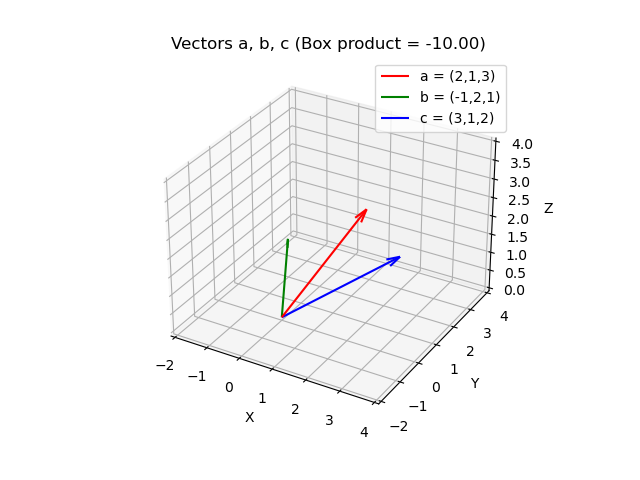
\includegraphics[width=0.6\columnwidth]{figs/vectors.png} 
   \caption*{Fig : Vectors}
  \label{Fig1}
\end{figure}

\end{frame}

\section*{Appendix: Code}

% C program
\begin{frame}[fragile]{C Code: points.c}
\begin{lstlisting}[language=C]

#include <math.h>
#include <stdio.h>

// Function to compute dot product
double dot(double u[3], double v[3]) {
  return u[0] * v[0] + u[1] * v[1] + u[2] * v[2];
}

// Function to compute determinant of 3x3 matrix
double det3(double M[3][3]) {
  return M[0][0] * (M[1][1] * M[2][2] - M[1][2] * M[2][1]) -
         M[0][1] * (M[1][0] * M[2][2] - M[1][2] * M[2][0]) +
         M[0][2] * (M[1][0] * M[2][1] - M[1][1] * M[2][0]);
}

// Function to compute box product using Gram matrix
double box_product() {
  double a[3] = {2, 1, 3};
  double b[3] = {-1, 2, 1};
  double c[3] = {3, 1, 2};

  double G[3][3] = {{dot(a, a), dot(a, b), dot(a, c)},
                    {dot(b, a), dot(b, b), dot(b, c)},
                    {dot(c, a), dot(c, b), dot(c, c)}};

  double detG = det3(G);

  // Negative since left-handed system
  double box = -sqrt(detG);

  return box;
}

\end{lstlisting}
\end{frame}

% Python calling C
\begin{frame}[fragile]{Python: call\_c.py}
\begin{lstlisting}[language=Python]

import sys
import ctypes
import numpy as np
import matplotlib.pyplot as plt
from mpl_toolkits.mplot3d import Axes3D

# Load shared object
lib = ctypes.CDLL("./points.so")
lib.box_product.restype = ctypes.c_double

# Call the C function
box = lib.box_product()
print("Box product (from C) =", box)

# Define vectors
a = np.array([2,1,3])
b = np.array([-1,2,1])
c = np.array([3,1,2])

# 3D plot
fig = plt.figure()
ax = fig.add_subplot(111, projection='3d')

# Origin
origin = np.array([0,0,0])

# Plot vectors with arrowheads
ax.quiver(*origin, *a, color='r', arrow_length_ratio=0.1, label="a = (2,1,3)")
ax.quiver(*origin, *b, color='g', arrow_length_ratio=0.1, label="b = (-1,2,1)")
ax.quiver(*origin, *c, color='b', arrow_length_ratio=0.1, label="c = (3,1,2)")

\end{lstlisting}
\end{frame}

\begin{frame}[fragile]{Python: call\_c.py}
\begin{lstlisting}[language=Python]

# Set limits
ax.set_xlim([-2,4])
ax.set_ylim([-2,4])
ax.set_zlim([0,4])

ax.set_xlabel("X")
ax.set_ylabel("Y")
ax.set_zlabel("Z")
ax.set_title(f"Vectors a, b, c (Box product = {box:.2f})")
ax.legend()

plt.savefig("vectors.png")
plt.show()

\end{lstlisting}
\end{frame}

\begin{frame}[fragile]{Python: plot.py}
\begin{lstlisting}[language=Python]

import numpy as np
import matplotlib.pyplot as plt
from mpl_toolkits.mplot3d import Axes3D

# Vectors
a = np.array([2,1,3])
b = np.array([-1,2,1])
c = np.array([3,1,2])

# Gram matrix
G = np.array([
    [np.dot(a,a), np.dot(a,b), np.dot(a,c)],
    [np.dot(b,a), np.dot(b,b), np.dot(b,c)],
    [np.dot(c,a), np.dot(c,b), np.dot(c,c)]
])

# Determinant and box product
detG = np.linalg.det(G)
box = -np.sqrt(detG)

print("Determinant of Gram matrix =", detG)
print("Box product =", box)

# 3D plot
fig = plt.figure()
ax = fig.add_subplot(111, projection='3d')

origin = np.array([0,0,0])

\end{lstlisting}
\end{frame}

\begin{frame}[fragile]{Python: plot.py}
\begin{lstlisting}[language=Python]


# Plot vectors
ax.quiver(*origin, *a, color='r', arrow_length_ratio=0.1, label="a = (2,1,3)")
ax.quiver(*origin, *b, color='g', arrow_length_ratio=0.1, label="b = (-1,2,1)")
ax.quiver(*origin, *c, color='b', arrow_length_ratio=0.1, label="c = (3,1,2)")

ax.set_xlim([-2,4])
ax.set_ylim([-2,4])
ax.set_zlim([0,4])

ax.set_xlabel("X")
ax.set_ylabel("Y")
ax.set_zlabel("Z")
ax.set_title(f"Vectors a, b, c (Box product = {box:.2f})")
ax.legend()

plt.savefig("vectors.png")
plt.show()


\end{lstlisting}
\end{frame}


\end{document}
